% ============================================================
%  CAPÍTULO 4 — METODOLOGÍA DE DESARROLLO
%  TFG: GlucoMate — Aplicación de Monitorización Continua de Glucosa
%  Ingeniería de Software
% ============================================================

\chapter{Metodología de Desarrollo}
\label{cap:metodologia}

Este capítulo describe el proceso de trabajo seguido durante el desarrollo de GlucoMate:
la metodología ágil aplicada, el modelo de ramificación de Git, la convención de mensajes
de \textit{commit}, las buenas prácticas de ingeniería de software adoptadas y las
herramientas seleccionadas en cada capa del sistema, justificando cada decisión.

% ──────────────────────────────────────────────────────────────
\section{Planificación temporal del proyecto}
\label{sec:gantt-proyecto}

\begin{figure}[H]
    \centering
    \resizebox{\textwidth}{!}{%
    \begin{ganttchart}[
        hgrid,
        vgrid,
        time slot format=isodate,
        x unit=0.15cm,
        y unit title=0.55cm,
        y unit chart=0.95cm,
        bar height=0.55,
        title height=1,
        title label font=\scriptsize\bfseries,
        bar label font=\small,
        bar label node/.append style={align=left,text width=4.8cm},
        bar/.append style={fill=blue!45,draw=blue!70!black},
        title/.append style={fill=gray!15},
        canvas/.append style={fill=white}
    ]{2026-01-01}{2026-05-10}
        \gantttitlecalendar{year, month=name, week} \\
        \ganttbar{\textbf{Inicio}\\\footnotesize 01/01/2026 -- 13/01/2026}{2026-01-01}{2026-01-13} \\
        \ganttbar{\textbf{Preparación}\\\footnotesize 14/01/2026 -- 01/02/2026}{2026-01-14}{2026-02-01} \\
        \ganttbar{\textbf{Ejecución}\\\footnotesize 02/02/2026 -- 07/04/2026}{2026-02-02}{2026-04-07} \\
        \ganttbar{\textbf{Documentación}\\\footnotesize 08/04/2026 -- 03/05/2026}{2026-04-08}{2026-05-03} \\
        \ganttbar{\textbf{Cierre / Entrega}\\\footnotesize 04/05/2026 -- 10/05/2026}{2026-05-04}{2026-05-10}
    \end{ganttchart}}
    \caption{Diagrama de Gantt del proyecto.}
    \label{fig:gantt-proyecto}
\end{figure}

El cronograma representado en la figura anterior se estructuró en cinco fases consecutivas, definidas para ordenar el desarrollo de GlucoMate de forma progresiva y asegurar una evolución controlada del proyecto desde la concepción inicial hasta la entrega final.

\subsection{Descripción de las fases}
\label{subsec:descripcion-fases-gantt}

\textbf{Inicio.} Esta fase se dedicó a la delimitación del alcance del trabajo, la concreción de los objetivos funcionales de la aplicación y la identificación de los principales retos técnicos, especialmente en torno a la lectura NFC del sensor y a la viabilidad general de la solución planteada.

\textbf{Preparación.} Durante esta etapa se establecieron las bases del proyecto: selección de tecnologías, definición de la arquitectura cliente-servidor, organización inicial del repositorio y preparación del entorno de trabajo necesario para abordar el desarrollo de la aplicación de forma ordenada.

\textbf{Ejecución.} En esta fase se concentró el grueso del trabajo técnico, incluyendo la implementación de la lectura NFC, el desarrollo del backend y la base de datos, la construcción de la interfaz móvil, la visualización de datos glucémicos y la integración del agente de inteligencia artificial.

\textbf{Documentación.} Una vez estabilizada la implementación principal, se abordó la redacción sistemática de la memoria, recogiendo las decisiones metodológicas y técnicas adoptadas, la descripción de la solución desarrollada y los resultados obtenidos durante las pruebas.

\textbf{Cierre / Entrega.} La fase final se orientó a la revisión global del proyecto, la corrección de detalles pendientes, la validación del material entregable y la preparación de la versión definitiva de la memoria y de los elementos necesarios para la presentación académica.

% ──────────────────────────────────────────────────────────────
\section{Desglose de costes del proyecto}
\label{sec:desglose-costes}

El presente apartado no se plantea como una factura ni como una oferta comercial emitida por
un proveedor, sino como un \textbf{desglose técnico de costes} asociado al desarrollo del
proyecto \textit{GlucoMate}. La estimación se ha realizado tomando como referencia directa el
diagrama de Gantt de la figura~\ref{fig:gantt-proyecto}, considerando la participación de
\textbf{un único desarrollador con perfil medio} y diferenciando entre el escenario realmente
ejecutado en Android y el escenario ampliado que habría sido necesario en caso de completar
también el desarrollo sobre iOS.

Para que la estimación resulte profesional y comparable, se distinguen dos tipos de importe:
por un lado, el \textbf{coste de adquisición} del equipamiento o dispositivo y, por otro, el
\textbf{coste imputable al proyecto}, entendido como la parte proporcional atribuible al periodo
 efectivo de trabajo. En el caso de los equipos informáticos se ha supuesto una vida útil de
36 meses, mientras que para los teléfonos móviles se ha considerado una vida útil de 24 meses.

El criterio de cálculo seguido para cada adquisición ha sido el de \textbf{amortización lineal
prorrateada por el tiempo de uso del proyecto}. En términos generales, el importe asignado a
GlucoMate se obtiene mediante la expresión:

\begin{equation}
    \text{Coste asignado al proyecto} = \frac{\text{Coste de adquisición}}{\text{Vida útil estimada en meses}} \times \text{Meses de duración del proyecto}
\end{equation}

En esta estimación, la duración tomada como referencia es la del cronograma completo del
proyecto, es decir, \textbf{130 días naturales}, equivalentes aproximadamente a
\textbf{4,27 meses}. De este modo, no se imputa el coste íntegro del dispositivo al trabajo,
sino únicamente la fracción de uso que razonablemente corresponde al periodo de desarrollo.

\subsection{Base temporal de la estimación}

El cronograma del proyecto abarca desde el 01/01/2026 hasta el 10/05/2026, lo que equivale a
\textbf{130 días naturales de trabajo planificado}. A partir de esa planificación, el reparto
temporal empleado para imputar el coste del desarrollo es el siguiente:

\begin{table}[H]
    \centering
    \caption{Distribución temporal y coste del desarrollo por fases.}
    \label{tab:coste-fases}
    \begin{tabular}{|p{4.2cm}|c|r|}
        \hline
        \textbf{Fase} & \textbf{Duración} & \textbf{Coste imputado} \\
        \hline
        Inicio & 13 días & 1.631,00 \euro{} \\
        \hline
        Preparación & 19 días & 2.383,77 \euro{} \\
        \hline
        Ejecución & 65 días & 8.155,00 \euro{} \\
        \hline
        Documentación & 26 días & 3.262,00 \euro{} \\
        \hline
        Cierre / Entrega & 7 días & 878,23 \euro{} \\
        \hline
        \textbf{Total personal} & \textbf{130 días} & \textbf{16.310,00 \euro{}} \\
        \hline
    \end{tabular}
\end{table}

Esta partida toma como referencia el coste de un \textbf{desarrollador de software de perfil
medio con titulación en Ingeniería Informática}, valorado a coste empresa en
\textbf{3.793,00 \euro{}/mes}. Dado que la planificación completa cubre aproximadamente 4,3
meses, el coste total de personal asciende a \textbf{16.310,00 \euro{}}.

En el caso del personal, el criterio es distinto al de los equipos, ya que no se trata de una
adquisición amortizable sino de \textbf{coste directo de dedicación}. Por ello, el cálculo se ha
realizado multiplicando el coste mensual estimado del perfil profesional por la duración total
del proyecto: \textbf{3.793,00 \euro{}/mes $\times$ 4,30 meses = 16.310,00 \euro{}}.

\subsection{Escenario realmente ejecutado: desarrollo Android}

En el escenario efectivamente llevado a cabo, el proyecto requirió un dispositivo Android para
la integración NFC, un equipo Windows como estación principal de desarrollo y sensores
FreeStyle Libre 2 Plus para validar el flujo real de lectura durante la fase de desarrollo.

\begin{table}[H]
    \centering
    \caption{Desglose de costes del escenario ejecutado en Android.}
    \label{tab:costes-android}
    \begin{tabular}{|p{6.2cm}|r|r|}
        \hline
        \textbf{Concepto} & \textbf{Adquisición} & \textbf{Imputable al proyecto} \\
        \hline
        Desarrollador perfil medio & --- & 16.310,00 \euro{} \\
        \hline
        Dispositivo Android con NFC & 449,00 \euro{} & 79,90 \euro{} \\
        \hline
        PC Windows de desarrollo & 799,00 \euro{} & 94,79 \euro{} \\
        \hline
        Sensores FreeStyle Libre 2 Plus & 630,00 \euro{} & 630,00 \euro{} \\
        \hline
        \textbf{Total escenario Android} & --- & \textbf{17.114,69 \euro{}} \\
        \hline
    \end{tabular}
\end{table}

La partida de sensores se ha calculado considerando que durante la \textbf{fase efectiva de
desarrollo técnico} ---desde la fase de inicio hasta la finalización de la ejecución--- se
cubrieron \textbf{97 días}, lo que implica la necesidad de \textbf{7 sensores} de 14 días de
duración. Tomando como base un coste unitario de \textbf{90,00 \euro{}} por sensor, el importe
total de consumibles asciende a \textbf{630,00 \euro{}}.

De forma más concreta, el valor imputado a cada adquisición del escenario Android se ha
obtenido así:

\begin{itemize}
    \item \textbf{Dispositivo Android con NFC.} Se ha tomado un coste de adquisición de
          \textbf{449,00 \euro{}} y una vida útil de \textbf{24 meses}. Aplicando el
          prorrateo temporal del proyecto, el cálculo resulta:
          \textbf{(449,00 / 24) $\times$ 4,27 = 79,90 \euro{}}.
    \item \textbf{PC Windows de desarrollo.} Se ha considerado un coste de adquisición de
          \textbf{799,00 \euro{}} y una vida útil de \textbf{36 meses}. El coste asignado al
          proyecto se obtiene como:
          \textbf{(799,00 / 36) $\times$ 4,27 = 94,79 \euro{}}.
    \item \textbf{Sensores FreeStyle Libre 2 Plus.} Al tratarse de un consumible, no se ha
          aplicado amortización, sino consumo real durante el desarrollo. El cálculo seguido
          ha sido: \textbf{97 días / 14 días por sensor = 6,93}, redondeado a
          \textbf{7 sensores}; por tanto,
          \textbf{7 $\times$ 90,00 \euro{} = 630,00 \euro{}}.
\end{itemize}

\subsection{Escenario ampliado: coste necesario si también se hubiese desarrollado en iOS}

Aunque la implementación final no se completó sobre iPhone, sí existió una fase de intento y
análisis de viabilidad. Por ello, resulta pertinente reflejar el coste adicional que habría
sido necesario asumir para completar el desarrollo, pruebas y posible distribución en el
ecosistema de Apple.

\begin{table}[H]
    \centering
    \caption{Coste incremental asociado a un desarrollo adicional en iOS.}
    \label{tab:costes-ios}
    \begin{tabular}{|p{6.2cm}|r|r|}
        \hline
        \textbf{Concepto} & \textbf{Adquisición} & \textbf{Imputable al proyecto} \\
        \hline
        Dispositivo iPhone para pruebas & 709,00 \euro{} & 126,17 \euro{} \\
        \hline
        Equipo Mac para compilación y firma & 719,00 \euro{} & 85,30 \euro{} \\
        \hline
        Programa Apple Developer & 99,00 \euro{} & 99,00 \euro{} \\
        \hline
        \textbf{Incremento total por iOS} & --- & \textbf{310,47 \euro{}} \\
        \hline
    \end{tabular}
\end{table}

La inclusión de esta partida responde a una limitación objetiva del ecosistema iOS: para
compilar, firmar y desplegar una aplicación en dispositivos Apple es necesario disponer de un
equipo macOS y de una cuenta de desarrollador activa. Por tanto, aun cuando el proyecto se ha
materializado finalmente sobre Android, el esfuerzo de extensión a iOS no podría considerarse
realista sin contemplar este sobrecoste específico.

Del mismo modo, el importe asignado al escenario iOS se ha estimado con el mismo criterio:

\begin{itemize}
    \item \textbf{Dispositivo iPhone para pruebas.} Considerando un coste de adquisición de
          \textbf{709,00 \euro{}} y una vida útil de \textbf{24 meses}, el coste asignado al
          proyecto sería:
          \textbf{(709,00 / 24) $\times$ 4,27 = 126,17 \euro{}}.
    \item \textbf{Equipo Mac para compilación y firma.} Para un coste de adquisición de
          \textbf{719,00 \euro{}} y una vida útil de \textbf{36 meses}, el prorrateo conduce a:
          \textbf{(719,00 / 36) $\times$ 4,27 = 85,30 \euro{}}.
    \item \textbf{Programa Apple Developer.} En este caso no se ha aplicado prorrateo, ya que
          se trata de una suscripción anual necesaria para la publicación y prueba sobre iOS.
          Por prudencia, se ha considerado el \textbf{coste completo anual de 99,00 \euro{}}
          como coste atribuible al proyecto.
\end{itemize}

\subsection{Resumen económico final}

Tomando como referencia exclusivamente el escenario ejecutado, el \textbf{coste total imputable
al proyecto GlucoMate} asciende a \textbf{17.114,69 \euro{}}. Si además se incorpora el
escenario complementario necesario para un desarrollo también operativo en iOS, el coste total
estimado pasaría a ser de \textbf{17.425,16 \euro{}}.

En consecuencia, puede afirmarse que la mayor parte del presupuesto se concentra en la
\textbf{dedicación técnica del desarrollador}, mientras que el hardware y los consumibles actúan
como costes de soporte necesarios para validar una solución que depende de lectura NFC real,
pruebas sobre dispositivos físicos y acceso continuado a sensores de glucosa durante el ciclo
de desarrollo.

% ──────────────────────────────────────────────────────────────
\section{Metodología ágil aplicada}
\label{sec:metodologia-agil}

El desarrollo de GlucoMate se ha llevado a cabo siguiendo los principios del
\textbf{desarrollo ágil} recogidos en el Manifiesto Ágil \cite{agilemanifesto2001},
adaptados a un proyecto individual de TFG. En lugar de establecer un plan rígido y
exhaustivo al inicio, el trabajo se organizó en \textbf{iteraciones cortas} —de
aproximadamente una semana de duración— en las que se priorizaba entregar un incremento
funcional y verificable del sistema al finalizar cada ciclo.

La gestión de las iteraciones no se apoyó en una herramienta externa de \textit{project
management}, sino en el propio historial de \textit{commits} del repositorio de GitHub,
que actúa como registro natural del avance del proyecto. Este enfoque es coherente con
proyectos pequeños donde la comunicación es unipersonal y la documentación formal de
\textit{sprints} añadiría burocracia sin valor real.

Las iteraciones cubrieron las siguientes fases, en el orden en que fueron completadas:

\begin{enumerate}
    \item \textbf{Prototipado de la lectura NFC.} Integración inicial de
          \texttt{react-native-nfc-manager}, verificación del protocolo ISO 15693 con el
          sensor Freestyle Libre 2 Plus y estudio de los comandos propietarios de Abbott.
    \item \textbf{Backend y persistencia.} Diseño del esquema de base de datos PostgreSQL,
          implementación de la API REST con Node.js/Express y verificación de los
          \textit{endpoints} de glucosa.
    \item \textbf{Gráfica D3.js.} Desarrollo del renderizado SVG de la curva histórica de
          doce horas y superposición de capas de eventos (insulina, comidas, ejercicio).
    \item \textbf{Módulos de eventos clínicos.} Implementación de los modales de registro
          de insulina, comidas y ejercicio, con sus respectivos \textit{endpoints} REST
          y lógica de transacciones en la base de datos.
    \item \textbf{Perfil de usuario.} Pantalla de configuración de los parámetros
          individuales de tratamiento (ICR, FSI, insulinas) y su persistencia mediante
          \textit{UPSERT}.
    \item \textbf{Agente de IA.} Diseño del \textit{system prompt} contextualizado,
          integración con la API de Groq para consumir el modelo
          \texttt{llama-3.3-70b-versatile}, lógica de reducción por deporte
          y mecanismo de reintento ante errores 503/429.
    \item \textbf{Integración y pulido.} Conexión de todos los módulos en la aplicación
          final, ajuste de la interfaz de usuario, corrección de errores detectados en
          las pruebas con sensor real y preparación del \textit{build} de producción.
\end{enumerate}

% ──────────────────────────────────────────────────────────────
\section{Control de versiones con Git y GitHub}
\label{sec:git-workflow}

Todo el código fuente de GlucoMate está alojado en un repositorio público de
\textbf{GitHub} (\url{https://github.com/manortgar/GlucoMate}). El uso de Git como
sistema de control de versiones distribuido ha permitido mantener un historial completo
y auditable de la evolución del proyecto, revertir cambios cuando una experimentación
no ha funcionado y separar el trabajo estable del trabajo en curso.

\subsection{Workflow de ramas: \textit{develop} y \textit{master}}
\label{subsec:branch-workflow}

El proyecto sigue un modelo de ramificación basado en dos ramas permanentes, inspirado
en el \textbf{Git Flow} \cite{driessen2010gitflow} simplificado:

\begin{itemize}
    \item \textbf{\texttt{master}} (rama principal): contiene exclusivamente código
          estable y verificado. Cada \textit{merge} sobre \texttt{master} representa
          una versión del sistema que ha sido probada funcionalmente y que podría ser
          distribuida. Esta rama es la que se compila con EAS Build para generar el
          APK de producción.

    \item \textbf{\texttt{develop}} (rama de desarrollo): es la rama de integración
          continua. Todo el trabajo nuevo —nuevas funcionalidades, correcciones y
          experimentos— se desarrolla directamente sobre \texttt{develop}. Cuando una funcionalidad es considerada
          completa y estable, se integra en \texttt{master} mediante un \textit{merge}.
\end{itemize}

Este modelo, aunque sencillo, introduce una separación clara entre el código de
producción y el código en desarrollo, lo que evita el antipatrón habitual en proyectos
académicos de trabajar directamente sobre \texttt{main} y perder la trazabilidad
del proceso.

La figura~\ref{fig:git-workflow} ilustra el flujo de trabajo entre ambas ramas.

\begin{figure}[H]
    \centering
    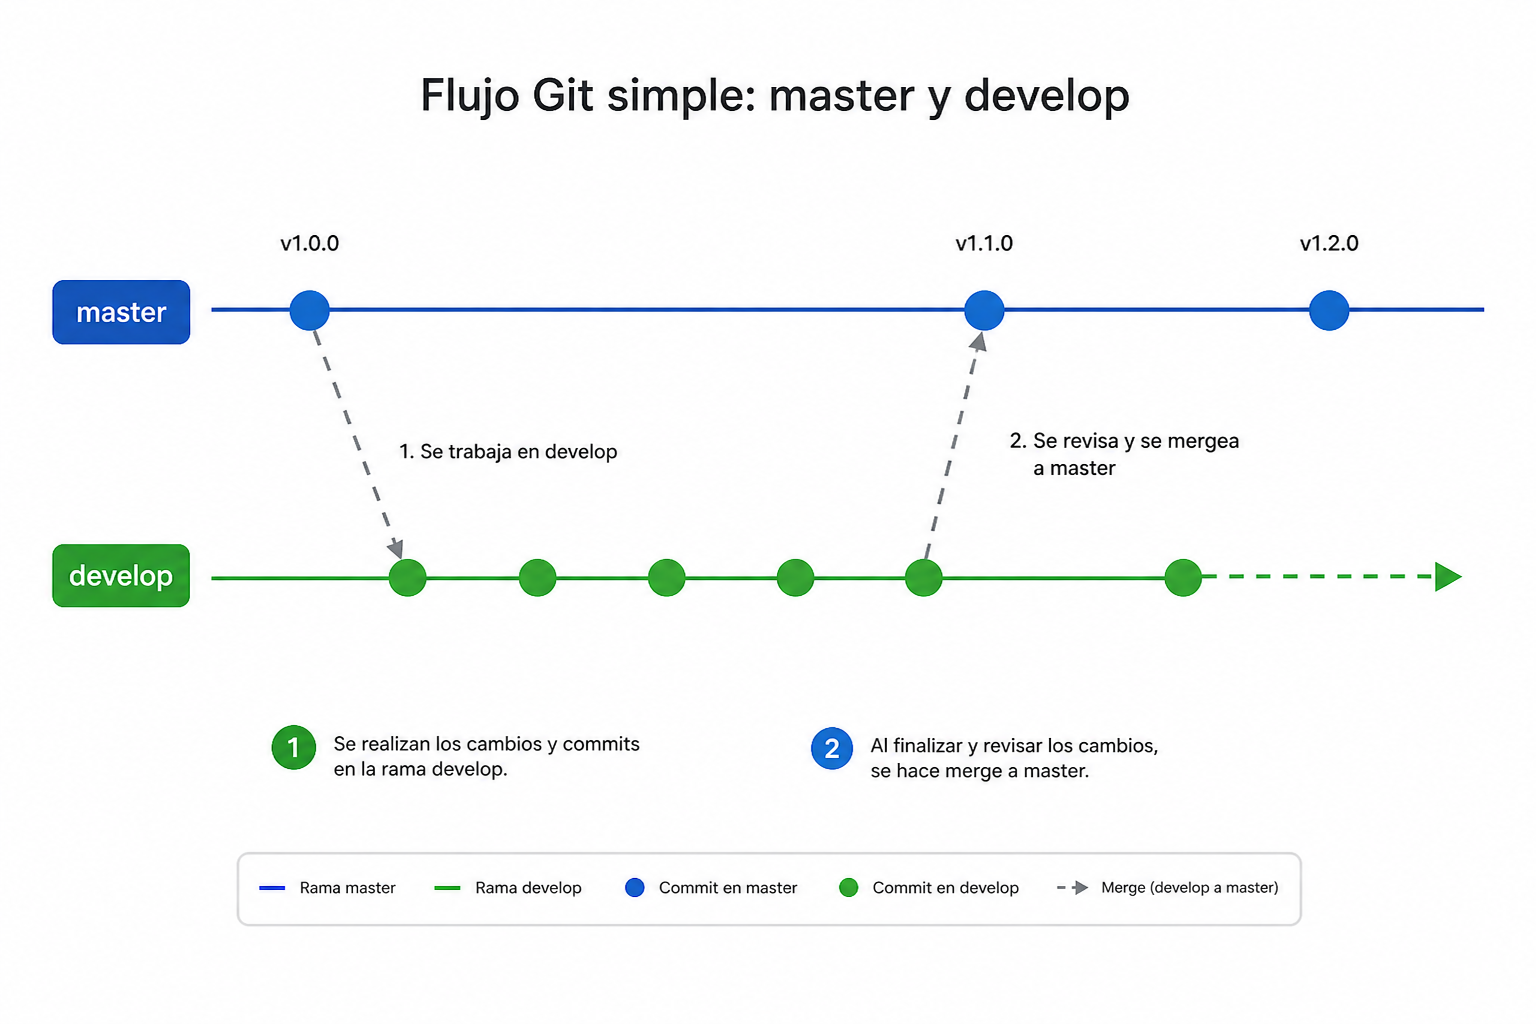
\includegraphics[width=0.95\textwidth]{figures/figura_4_1_workflow.png}
    \caption{Modelo de ramificación utilizado en GlucoMate: rama \texttt{develop} para
             integración continua y \texttt{master} para versiones estables.}
    \label{fig:git-workflow}
\end{figure}

% ──────────────────────────────────────────────────────────────
\section{Conventional Commits}
\label{sec:conventional-commits}

Para garantizar que el historial de \textit{commits} sea legible, semántico y
automáticamente procesable, todos los mensajes de confirmación de cambios siguen la
especificación \textbf{Conventional Commits} \cite{conventionalcommits}, una convención
ampliamente adoptada en la industria del software.

\subsection{Estructura del mensaje}

Cada mensaje de \textit{commit} responde a la siguiente estructura:

\begin{verbatim}
<tipo>(<ámbito>): <descripción breve>

[cuerpo opcional]

[notas de pie opcionales]
\end{verbatim}

\noindent Donde \texttt{<tipo>} es uno de los valores definidos por la especificación:

\begin{table}[H]
\centering
\caption{Tipos de \textit{commit} utilizados en GlucoMate según la especificación
         Conventional Commits.}
\label{tab:commit-types}
\begin{tabular}{|l|p{9.5cm}|}
\hline
\textbf{Tipo} & \textbf{Significado} \\
\hline
\texttt{feat}     & Añade una nueva funcionalidad al sistema. \\
\texttt{fix}      & Corrige un error o comportamiento incorrecto. \\
\texttt{refactor} & Reestructura código sin cambiar su comportamiento externo. \\
\texttt{docs}     & Cambios exclusivamente en la documentación. \\
\texttt{style}    & Ajustes de formato, sangría o estilo sin impacto funcional. \\
\texttt{chore}    & Tareas de mantenimiento: actualización de dependencias, configuración. \\
\texttt{test}     & Adición o modificación de pruebas. \\
\texttt{perf}     & Mejora del rendimiento de algún componente. \\
\hline
\end{tabular}
\end{table}

\subsection{Ejemplos representativos del proyecto}

A continuación se recogen mensajes de \textit{commit} reales del historial de GlucoMate
que ilustran la aplicación de esta convención:

\begin{verbatim}
fix(ui): corregir posición inicial del trazado en la gráfica.
feat(ui): implementar e integrar el modal de registro de insulina.
feat(api): añadir endpoints para gestionar eventos de insulina.
chore: actualizar dependencias en package.json.
feat(ui): añadir assets para los botones de acción.
Merge pull request #2 from manortgar/develop
chore: actualizar .gitignore
fix(ui): ajustar dimensiones de pantalla al área segura de Android.
Merge pull request #1 from manortgar/develop
feat(ui): implementa vista de Mi Perfil de usuario y nueva ruta.
chore(brand): cambiar nombre de la aplicación e icono.
feat(api): añadir nuevos endpoints para la gestión de Mi Perfil.
\end{verbatim}

\subsection{Beneficios obtenidos}

La adopción de esta convención ha aportado tres beneficios concretos al proyecto:

\begin{enumerate}
    \item \textbf{Legibilidad del historial.} Cualquier persona que consulte el
          repositorio puede entender qué cambió, en qué capa del sistema y con qué
          intención, sin necesidad de leer el \textit{diff} completo.

    \item \textbf{Generación automática de \textit{changelogs}.} Herramientas como
          \texttt{standard-version} o \texttt{release-please} pueden generar un
          registro de cambios estructurado a partir de los mensajes de \textit{commit},
          lo que facilitará las versiones futuras de la aplicación.

    \item \textbf{Disciplina de desarrollo.} La obligación de clasificar cada
          \textit{commit} fuerza al desarrollador a realizar cambios atómicos y con
          una responsabilidad clara, evitando los \textit{commits} de tipo
          ``arreglos varios'' que dificultan la revisión y la depuración.
\end{enumerate}

% ──────────────────────────────────────────────────────────────
\section{Buenas prácticas aplicadas}
\label{sec:buenas-practicas}

Más allá del control de versiones, el desarrollo de GlucoMate ha incorporado un conjunto
de buenas prácticas de ingeniería de software que se describen a continuación.

\subsection{Separación de responsabilidades: arquitectura cliente-servidor}
\label{subsec:separacion-responsabilidades}

El sistema está dividido en dos capas claramente diferenciadas —\textbf{frontend} y
\textbf{backend}— que se comunican exclusivamente a través de una API REST documentada.
Esta separación garantiza que:

\begin{itemize}
    \item La lógica de negocio (cálculo de IOB, integración con Groq y
          \texttt{llama-3.3-70b-versatile}, gestión de transacciones en base de datos)
          reside en el servidor, donde puede ser
          mantenida y actualizada sin redistribuir la aplicación móvil.
    \item El cliente móvil se limita a presentar datos y gestionar la interacción con el
          usuario, sin acoplar lógica de dominio en los componentes de interfaz.
    \item Ambas capas pueden evolucionar de forma independiente: un futuro cliente web
          o iOS podría consumir la misma API sin modificar el backend.
\end{itemize}

\subsection{Modularidad y cohesión}
\label{subsec:modularidad}

El frontend está organizado en componentes React Native con responsabilidades únicas y
bien definidas:

\begin{itemize}
    \item \textbf{\texttt{NFCScanner.js}}: pantalla principal. Gestiona el estado global
          de la aplicación (lectura NFC, historial, eventos activos) y orquesta el
          renderizado de la gráfica y los módulos de acción.
    \item \textbf{\texttt{ChatModal.js}}: interfaz de conversación con el agente de IA.
          Completamente autocontenido, recibe \texttt{backendUrl} como argumento y gestiona
          su propio estado de mensajes y carga.
    \item \textbf{\texttt{InsulinModal.js}, \texttt{FoodModal.js},
          \texttt{ExerciseModal.js}}: modales de registro de eventos clínicos. Cada uno
          encapsula su formulario, validación y llamada al \textit{endpoint} correspondiente.
    \item \textbf{\texttt{ProfileScreen.js}}: pantalla de perfil. Independiente del flujo
          principal, gestiona la carga y persistencia del perfil de tratamiento.
\end{itemize}

En el backend, la separación entre \texttt{server.js} (lógica de rutas y controladores)
y \texttt{db.js} (gestión del \textit{pool} de conexiones a PostgreSQL) sigue el principio
de responsabilidad única (SRP) y facilita la sustitución del motor de base de datos sin
tocar la lógica de negocio.

\subsection{Gestión de errores y resiliencia}
\label{subsec:gestion-errores}

El backend implementa un mecanismo de \textbf{reintento con espera exponencial} para las
llamadas a la API de Groq, dado que este servicio puede responder con errores 503
(\textit{Service Unavailable}) o 429 (\textit{Too Many Requests}) bajo carga. El
algoritmo realiza hasta tres intentos con una pausa de cinco segundos entre ellos antes
de propagar el error al cliente:

\begin{lstlisting}[language=JavaScript, caption={Mecanismo de reintento con espera exponencial
para las llamadas a la API de Groq}, label={cod:error-ia}, captionpos=b]
let retries = 3;
while (retries > 0 && !success) {
    try {
        response = await ai.models.generateContent({ ... });
        success = true;
    } catch (err) {
        if ((err.status === 503 || err.status === 429) && retries > 1) {
            retries--;
            await new Promise(resolve => setTimeout(resolve, 5000));
        } else {
            throw err;
        }
    }
}
\end{lstlisting}

Adicionalmente, todas las rutas del backend están envueltas en bloques \texttt{try/catch}
que devuelven respuestas HTTP con códigos de estado apropiados (400, 500) y mensajes
descriptivos, evitando que un error interno exponga información sensible del sistema.

Las operaciones que implican múltiples escrituras en la base de datos —como el registro
de una comida con bolo de insulina asociado— se ejecutan dentro de
\textbf{transacciones ACID} con \texttt{BEGIN}/\texttt{COMMIT}/\texttt{ROLLBACK},
garantizando la consistencia de los datos ante fallos parciales.

\subsection{Variables de entorno y seguridad de credenciales}
\label{subsec:env-vars}

Las credenciales sensibles del sistema (clave de API de Groq, contraseña de PostgreSQL,
host y puerto de la base de datos) se gestionan mediante \textbf{variables de entorno}
cargadas con la librería \texttt{dotenv}. El fichero \texttt{.env} está incluido en
\texttt{.gitignore} para garantizar que nunca se publique en el repositorio:

\begin{verbatim}
# .env (nunca versionado)
GROQ_API_KEY=gsk_...
DB_USER=postgres
DB_PASSWORD=...
DB_NAME=glucose_db
DB_HOST=localhost
DB_PORT=5432
\end{verbatim}

Esta práctica es especialmente crítica en proyectos que integran APIs de terceros con
facturación por uso, donde una clave comprometida podría derivar en costes económicos
significativos.

\subsection{Arquitectura de la API REST}
\label{subsec:api-rest}

Los \textit{endpoints} del backend siguen las convenciones REST estándar: sustantivos
en plural para los recursos, verbos HTTP semánticos (\texttt{GET} para consulta,
\texttt{POST} para creación, \texttt{PUT} para actualización completa) y códigos de
estado HTTP coherentes con el resultado de cada operación (201 para creación exitosa,
400 para validación fallida, 500 para error interno). Esta consistencia facilita el
consumo de la API desde el cliente y, en el futuro, desde cualquier otra aplicación.

% ──────────────────────────────────────────────────────────────
\section{Gestión de dependencias con npm y build con EAS}
\label{sec:herramientas}

La selección de tecnologías ha respondido a tres criterios: adecuación técnica al
problema, madurez del ecosistema y productividad en un contexto de desarrollo individual.

\subsection{React Native con Expo}
\label{subsec:herramienta-rn}

\textbf{React Native} \cite{facebook2015reactnative} es un \textit{framework} de código
abierto desarrollado por Meta que permite construir aplicaciones móviles nativas para
Android e iOS utilizando JavaScript y el paradigma de componentes de React. A diferencia
de las soluciones de \textit{webview} (como Ionic o Cordova), React Native compila los
componentes a elementos de interfaz nativos de cada plataforma, lo que proporciona
rendimiento y aspecto visual indistinguibles de una aplicación nativa.

La elección de React Native sobre alternativas como Flutter o el desarrollo nativo en
Kotlin/Java se justifica por:

\begin{itemize}
    \item La disponibilidad de \texttt{react-native-nfc-manager}, una librería madura
          que abstrae el acceso a la pila NFC del sistema operativo Android y soporta el
          protocolo ISO 15693 (NfcV) necesario para comunicarse con el sensor Freestyle
          Libre.
    \item El ecosistema JavaScript compartido con el backend (Node.js), que reduce la
          carga cognitiva de cambiar de lenguaje entre capas.
    \item La reutilización de librerías de visualización como D3.js, cuyo ecosistema es
          incomparablemente más rico en JavaScript que en Dart o Kotlin.
\end{itemize}

\textbf{Expo} \cite{expo2020} es una plataforma construida sobre React Native que
simplifica la configuración del entorno de desarrollo, la gestión de permisos del sistema
operativo (NFC, cámara, etc.) y el proceso de compilación. En GlucoMate se utiliza con
la configuración \texttt{expo-dev-client}, que permite generar una aplicación de
desarrollo personalizada con acceso completo a las APIs nativas, superando las
limitaciones de la versión estándar de Expo Go para funcionalidades como NFC.

\subsection{Build de producción con EAS Build}
\label{subsec:herramienta-eas}

\textbf{EAS Build} (Expo Application Services Build) \cite{eas2021} es el servicio de
compilación en la nube de Expo. Permite generar el APK o AAB de producción de la
aplicación Android sin necesidad de tener instalado Android Studio ni el SDK de Android
en la máquina local. La configuración del proyecto en \texttt{eas.json} define los
perfiles de compilación (\textit{development}, \textit{preview}, \textit{production})
con sus respectivas opciones de firma y distribución.

La justificación de EAS Build frente a la compilación local es doble: elimina la
complejidad de mantener una cadena de compilación nativa en el entorno de desarrollo y
garantiza reproducibilidad en entornos limpios y controlados.

\subsection{Gestión de dependencias con npm}
\label{subsec:herramienta-npm}

\textbf{npm} (\textit{Node Package Manager}) \cite{npm2010} es el gestor de paquetes
estándar del ecosistema JavaScript, utilizado tanto en el frontend como en el backend. El
fichero \texttt{package-lock.json} garantiza que las instalaciones sean reproducibles,
fijando las versiones exactas de todas las dependencias transitivas. Entre las bibliotecas
más relevantes del frontend se encuentran \texttt{react-native-nfc-manager} para el acceso
al hardware NFC, \texttt{d3-shape} y \texttt{d3-scale} para la representación de curvas y
escalas temporales, \texttt{react-native-svg} para el renderizado gráfico y
\texttt{@react-navigation/bottom-tabs} para la navegación principal de la aplicación.

En el backend, las dependencias clave incluyen \texttt{express} como marco HTTP,
\texttt{pg} para la conexión con PostgreSQL, el SDK de Groq para el acceso al modelo
\texttt{llama-3.3-70b-versatile}, además de utilidades como \texttt{dotenv} para la carga
de configuración y \texttt{cors} para habilitar la comunicación segura con el cliente móvil.

\subsection{Backend: Node.js con Express}
\label{subsec:herramienta-node}

\textbf{Node.js} \cite{nodejs2009} es un entorno de ejecución JavaScript asíncrono
basado en el motor V8 de Google Chrome, diseñado para construir aplicaciones de red
escalables. Su modelo de E/S no bloqueante mediante \textit{event loop} lo hace
especialmente adecuado para APIs REST que realizan operaciones de I/O intensivas
(consultas a base de datos, llamadas a APIs externas), que es exactamente el perfil
de carga de GlucoMate.

\textbf{Express} \cite{express2010} es el \textit{framework} HTTP minimalista más
utilizado en el ecosistema Node.js. Proporciona un sistema de enrutamiento, \textit{middleware}
y gestión de peticiones/respuestas HTTP con una superficie de API reducida, lo que facilita
la comprensión y el mantenimiento del código del servidor.

\subsection{Base de datos: PostgreSQL}
\label{subsec:herramienta-postgres}

\textbf{PostgreSQL} \cite{postgres1996} es el sistema de gestión de bases de datos
relacionales de código abierto más avanzado disponible. Su elección sobre alternativas
como SQLite o MySQL se justifica por:

\begin{itemize}
    \item \textbf{Soporte completo de ACID.} Las transacciones del backend que registran
          simultáneamente una comida y un bolo de insulina requieren garantías de
          atomicidad que SQLite no ofrece de forma robusta en escenarios concurrentes.
    \item \textbf{Tipos de datos ricos.} PostgreSQL soporta \texttt{TIMESTAMP WITH TIME
          ZONE}, \texttt{NUMERIC} y \texttt{INTERVAL} de forma nativa, lo que simplifica
          las consultas de ventana temporal (por ejemplo, ``lecturas de las últimas 12 horas'').
    \item \textbf{UPSERT nativo.} La instrucción \texttt{INSERT ... ON CONFLICT DO UPDATE}
          permite gestionar el perfil de usuario como una fila única que se crea o
          actualiza atómicamente, sin necesidad de lógica adicional en el servidor.
    \item \textbf{Escalabilidad futura.} Aunque en la versión actual el backend opera en
          red local, PostgreSQL está preparado para ser desplegado en entornos de
          producción en la nube (AWS RDS, Supabase) sin cambios en el esquema ni en el
          código de acceso a datos.
\end{itemize}

\subsection{Visualización: D3.js sobre SVG nativo}
\label{subsec:herramienta-d3}

\textbf{D3.js} (\textit{Data-Driven Documents}) \cite{bostock2011d3} es la librería de
visualización de datos más utilizada en el ecosistema JavaScript. En GlucoMate se emplean
específicamente los módulos \texttt{d3-scale} y \texttt{d3-shape}, que proporcionan:

\begin{itemize}
    \item \texttt{scaleTime()}: transforma marcas de tiempo Unix en coordenadas
          de píxel en el eje X, gestionando correctamente los cambios de horario y
          la aritmética de fechas.
    \item \texttt{scaleLinear()}: mapea los valores de glucosa (rango 50–300+ mg/dL)
          al eje Y del área de dibujo.
    \item \texttt{line().curve(curveMonotoneX)}: genera la ruta SVG de la curva
          interpolada con suavizado monotónico, que preserva la forma real de los datos
          sin introducir oscilaciones artificiales entre puntos.
\end{itemize}

La elección de D3.js sobre librerías de gráficas de alto nivel para React Native
(Victory Native, React Native Chart Kit) se justifica por el nivel de control que
requiere la gráfica de GlucoMate: la superposición de múltiples capas de información
(curva de glucosa, ventanas de insulina activa con línea de pico, ventanas de ejercicio
con zona de peligro postejercicio, marcadores de comidas) es una visualización altamente
personalizada que las librerías de gráficas estándar no permiten implementar sin
comprometer su API interna.

\subsection{Inteligencia Artificial: \texttt{llama-3.3-70b-versatile} en Groq}
\label{subsec:herramienta-llama-groq}

El agente de inteligencia artificial de GlucoMate está construido sobre
\textbf{\texttt{llama-3.3-70b-versatile}} \cite{groq2026llama}, un modelo de lenguaje
grande (LLM) servido a través de la API de Groq. La elección de esta combinación frente
a alternativas como GPT-4o (OpenAI) o Claude (Anthropic) se fundamenta en:

\begin{itemize}
    \item \textbf{Latencia.} Groq está orientado a inferencia de baja latencia,
          lo que es esencial en una aplicación móvil donde el usuario espera una
          respuesta en tiempo real.
    \item \textbf{Coste.} El acceso gratuito mediante una API key de Groq es suficiente para el
          volumen de consultas de un usuario individual, lo que hace viable el proyecto
          sin coste operativo.
    \item \textbf{Temperatura baja.} El modelo se configura con \texttt{temperature: 0.2},
          lo que reduce la variabilidad de las respuestas y favorece el razonamiento
          clínico estructurado frente a respuestas creativas.
\end{itemize}

La integración se realiza en el backend (no en el cliente móvil), lo que garantiza que
la clave de API nunca se expone en el código de la aplicación distribuida.

\subsection{Prototipado: mockups digitales}
\label{subsec:herramienta-prototipado}

El diseño de la interfaz de usuario se abordó mediante \textbf{mockups digitales de
alta fidelidad} antes de cerrar la implementación visual definitiva. Este enfoque
permitió validar con antelación la jerarquía visual, el reparto del espacio y la
consistencia cromática de la aplicación, además de comunicar con claridad la propuesta
de interfaz sin necesidad de desarrollar todavía todos los flujos funcionales.

Los mockups definieron las decisiones de diseño más importantes de la interfaz: la
disposición del valor de glucosa como elemento dominante en la parte superior de la
pantalla, la ubicación del botón NFC en la esquina superior izquierda para acceso rápido,
la fila de botones de acción rápida (comida, insulina, deporte) como acceso directo a
los modales de registro, la pantalla de perfil terapéutico para la configuración del
tratamiento y el acceso al chat de IA en posición secundaria pero visible.

Las Figuras~\ref{fig:mockups-ui-principales} y~\ref{fig:mockups-ui-secundarias}
recogen los mockups principales elaborados para el proyecto: la pantalla principal con
la curva glucémica, la vista de perfil terapéutico, los formularios de registro de
eventos y la interfaz conversacional del asistente.

\newcommand{\mockupcard}[2]{%
    \begin{tikzpicture}
        \node[inner sep=0pt, outer sep=0pt] (img) at (0,0)
            {\includegraphics[width=#1,height=0.36\textheight,keepaspectratio]{#2}};
        \begin{scope}
            \clip[rounded corners=7pt] (img.south west) rectangle (img.north east);
            \node[inner sep=0pt, outer sep=0pt, anchor=south west] at (img.south west)
                {\includegraphics[width=#1,height=0.36\textheight,keepaspectratio]{#2}};
        \end{scope}
        \draw[rounded corners=7pt, line width=0.45pt, draw=black!25]
            (img.south west) rectangle (img.north east);
    \end{tikzpicture}%
}

\begin{figure}[p]
    \centering
    \subfigure[Pantalla principal con lectura actual de glucosa, accesos rápidos y gráfica histórica.]{%
        \mockupcard{0.78\textwidth}{uploads/grafica4-3.png}}

    \vspace{1em}

    \subfigure[Pantalla de perfil terapéutico para la configuración de insulinas e ICR.]{%
        \mockupcard{0.78\textwidth}{uploads/perfil4-3.png}}
    \caption{Mockups principales de la interfaz de GlucoMate.}
    \label{fig:mockups-ui-principales}
\end{figure}

\begin{figure}[p]
    \centering
    \subfigure[Formularios de registro de comida, insulina y deporte mediante modales específicos.]{%
        \mockupcard{0.78\textwidth}{uploads/Copilot_20260510_131939.png}}

    \vspace{1em}

    \subfigure[Interfaz conversacional del asistente GlucoMate AI para apoyo y orientación contextual.]{%
        \mockupcard{0.78\textwidth}{uploads/chat4-3.png}}
    \caption{Mockups complementarios de interacción y asistencia inteligente.}
    \label{fig:mockups-ui-secundarias}
\end{figure}

% ──────────────────────────────────────────────────────────────
\section{Resumen}
\label{sec:metodologia-resumen}

La tabla~\ref{tab:resumen-metodologia} sintetiza las decisiones metodológicas y
tecnológicas más relevantes del proyecto.

\begin{table}[H]
\centering
\caption{Resumen de la metodología y tecnologías principales de GlucoMate.}
\label{tab:resumen-metodologia}
\begin{tabular}{|l|l|}
\hline
\textbf{Dimensión} & \textbf{Decisión adoptada} \\
\hline
Metodología       & Desarrollo ágil iterativo (iteraciones semanales) \\
Control versiones & Git + GitHub (\texttt{develop} / \texttt{master}) \\
Estilo de commits & Conventional Commits \\
Frontend          & React Native 0.81 + Expo 54 \\
Build nativo      & EAS Build (Expo Application Services) \\
Gestor paquetes   & npm + \texttt{package-lock.json} \\
Visualización     & D3.js (\texttt{d3-scale}, \texttt{d3-shape}) + react-native-svg \\
Backend           & Node.js + Express 5 \\
Base de datos     & PostgreSQL (pool de conexiones con \texttt{pg}) \\
IA generativa     & \texttt{llama-3.3-70b-versatile} (Groq, \texttt{temperature: 0.2}) \\
Seguridad         & Variables de entorno con \texttt{dotenv} \\
Prototipado UI    & Mockups digitales de alta fidelidad \\
Plataforma target & Android (API 24+) \\
\hline
\end{tabular}
\end{table}
